\documentclass[12pt, titlepage]{article}

\usepackage{fullpage}
\usepackage[round]{natbib}
\usepackage{multirow}
\usepackage{booktabs}
\usepackage{tabularx}
\usepackage{graphicx}
\usepackage{float}
\usepackage{hyperref}
\hypersetup{
    colorlinks,
    citecolor=blue,
    filecolor=black,
    linkcolor=red,
    urlcolor=blue
}

%% Comments

\usepackage{color}

\newif\ifcomments\commentstrue %displays comments
%\newif\ifcomments\commentsfalse %so that comments do not display

\ifcomments
\newcommand{\authornote}[3]{\textcolor{#1}{[#3 ---#2]}}
\newcommand{\todo}[1]{\textcolor{red}{[TODO: #1]}}
\else
\newcommand{\authornote}[3]{}
\newcommand{\todo}[1]{}
\fi

\newcommand{\wss}[1]{\authornote{blue}{SS}{#1}} 
\newcommand{\plt}[1]{\authornote{magenta}{TPLT}{#1}} %For explanation of the template
\newcommand{\an}[1]{\authornote{cyan}{Author}{#1}}

%% Common Parts

\newcommand{\progname}{Live Neuro} % PUT YOUR PROGRAM NAME HERE
\newcommand{\authname}{Bo Liang} % AUTHOR NAMES

\usepackage{hyperref}
    \hypersetup{colorlinks=true, linkcolor=blue, citecolor=blue, filecolor=blue,
                urlcolor=blue, unicode=false}
    \urlstyle{same}
                                


\newcounter{acnum}
\newcommand{\actheacnum}{AC\theacnum}
\newcommand{\acref}[1]{AC\ref{#1}}

\newcounter{ucnum}
\newcommand{\uctheucnum}{UC\theucnum}
\newcommand{\uref}[1]{UC\ref{#1}}

\newcounter{mnum}
\newcommand{\mthemnum}{M\themnum}
\newcommand{\mref}[1]{M\ref{#1}}

\begin{document}

\title{Module Guide for \progname{}}
\author{\authname}
\date{\today}

\maketitle

\pagenumbering{roman}

\section{Revision History}

\begin{tabularx}{\textwidth}{p{3cm}p{2cm}X}
\toprule {\bf Date} & {\bf Version} & {\bf Notes}\\
\midrule
March 17 2025 & 1.0 & initial draft\\
\bottomrule
\end{tabularx}

\newpage

\section{Reference Material}

This section records information for easy reference.

\subsection{Abbreviations and Acronyms}

\renewcommand{\arraystretch}{1.2}
\begin{tabular}{l l} 
  \toprule		
  \textbf{symbol} & \textbf{description}\\
  \midrule 
  AC & Anticipated Change\\
  DAG & Directed Acyclic Graph \\
  M & Module \\
  MG & Module Guide \\
  OS & Operating System \\
  R & Requirement\\
  SC & Scientific Computing \\
  SRS & Software Requirements Specification\\
  TRF & Temporal Response Function\\
  \progname & Explanation of program name\\
  UC & Unlikely Change \\
  \bottomrule
\end{tabular}\\

\newpage

\tableofcontents

\listoftables

\listoffigures

\newpage

\pagenumbering{arabic}

\section{Introduction}

Decomposing a system into modules is a commonly accepted approach to developing
software.  A module is a work assignment for a programmer or programming
team~\citep{ParnasEtAl1984}.  We advocate a decomposition
based on the principle of information hiding~\citep{Parnas1972a}.  This
principle supports design for change, because the ``secrets'' that each module
hides represent likely future changes.  Design for change is valuable in SC,
where modifications are frequent, especially during initial development as the
solution space is explored.  

Our design follows the rules layed out by \citet{ParnasEtAl1984}, as follows:
\begin{itemize}
\item System details that are likely to change independently should be the
  secrets of separate modules.
\item Each data structure is implemented in only one module.
\item Any other program that requires information stored in a module's data
  structures must obtain it by calling access programs belonging to that module.
\end{itemize}

After completing the first stage of the design, the Software Requirements
Specification (SRS), the Module Guide (MG) is developed~\citep{ParnasEtAl1984}. The MG
specifies the modular structure of the system and is intended to allow both
designers and maintainers to easily identify the parts of the software.  The
potential readers of this document are as follows:

\begin{itemize}
\item New project members: This document can be a guide for a new project member
  to easily understand the overall structure and quickly find the
  relevant modules they are searching for.
\item Maintainers: The hierarchical structure of the module guide improves the
  maintainers' understanding when they need to make changes to the system. It is
  important for a maintainer to update the relevant sections of the document
  after changes have been made.
\item Designers: Once the module guide has been written, it can be used to
  check for consistency, feasibility, and flexibility. Designers can verify the
  system in various ways, such as consistency among modules, feasibility of the
  decomposition, and flexibility of the design.
\end{itemize}

The rest of the document is organized as follows. Section
\ref{SecChange} lists the anticipated and unlikely changes of the software
requirements. Section \ref{SecMH} summarizes the module decomposition that
was constructed according to the likely changes. Section \ref{SecConnection}
specifies the connections between the software requirements and the
modules. Section \ref{SecMD} gives a detailed description of the
modules. Section \ref{SecTM} includes two traceability matrices. One checks
the completeness of the design against the requirements provided in the SRS. The
other shows the relation between anticipated changes and the modules. Section
\ref{SecUse} describes the use relation between modules.

\section{Anticipated and Unlikely Changes} \label{SecChange}
\subsection{Anticipated Changes} \label{SecAchange}

Anticipated changes are the source of the information that is to be hidden
inside the modules. Ideally, changing one of the anticipated changes will only
require changing the one module that hides the associated decision. The approach
adapted here is called design for
change.

\begin{description}
\item[\refstepcounter{acnum} \actheacnum \label{acHardware}:] Hardware platform (e.g., OS compatibility)
\item[\refstepcounter{acnum} \actheacnum \label{acInput}:] Input data format (e.g., MEG/EEG)
\item[\refstepcounter{acnum} \actheacnum \label{acVisualization}:] Visualization methods (e.g., 2D to 3D)
\item[\refstepcounter{acnum} \actheacnum \label{acInteraction}:] Interaction methods (e.g., click/slide/drag/zoom)
\end{description}


\subsection{Unlikely Changes} \label{SecUchange}

The module design should be as general as possible. However, a general system is
more complex. Sometimes this complexity is not necessary. Fixing some design
decisions at the system architecture stage can simplify the software design. If
these decision should later need to be changed, then many parts of the design
will potentially need to be modified. Hence, it is not intended that these
decisions will be changed.

\begin{description}
\item[\refstepcounter{ucnum} \uctheucnum \label{ucIO}:] Input/Output devices
  (Input: File(MEG/EEG data), Output: File(data image)).
\item [\refstepcounter{ucnum} \uctheucnum \label{ucCoreTRFmodel}:] Core TRF-based stimulus-response model.
\item
\end{description}

\section{Module Hierarchy} \label{SecMH}

This section provides an overview of the module design. Modules are summarized
in a hierarchy decomposed by secrets in Table \ref{TblMH}. The modules listed
below, which are leaves in the hierarchy tree, are the modules that will
actually be implemented.

\begin{description}
\item [\refstepcounter{mnum} \mthemnum \label{mHH}:] Hardware-Hiding Module
\item [\refstepcounter{mnum} \mthemnum \label{m2}:] Input Format Module
\item [\refstepcounter{mnum} \mthemnum \label{m3}:] Data Processing Module
\item [\refstepcounter{mnum} \mthemnum \label{m4}:] Visualization Module
\item [\refstepcounter{mnum} \mthemnum \label{m5}:] TRF Calculation Module
\end{description}

\begin{table}[h!]
\centering
\begin{tabular}{p{0.3\textwidth} p{0.5\textwidth}p{0.1\textwidth}}
\toprule
\textbf{Level 1} & \textbf{Level 2}& \textbf{Module ID}\\
\midrule

{Hardware-Hiding Module} &  Hardware-Hiding Module
 & M1 \\
\midrule

\multirow{3}{0.3\textwidth}{Behaviour-Hiding Module}
& Input Format Module & M2\\
& Data Processing Module & M3\\
& Visualization Module & M4\\

\midrule

\multirow{1}{0.3\textwidth}{Software Decision Module} & TRF Calculation Module & M5\\
\bottomrule

\end{tabular}
\caption{Module Hierarchy}
\label{TblMH}
\end{table}

\section{Connection Between Requirements and Design} \label{SecConnection}

The system is designed to fulfill the functional and non-functional requirements specified in the SRS. The following table traces requirements to their corresponding modules:

\begin{table}[h!]
\centering
\begin{tabular}{p{0.5\textwidth} p{0.3\textwidth}}
\toprule
\textbf{
Requirement (SRS)} &  \textbf{Module ID}\\
\midrule

{R1: Interactive visualization plots}
 & M1,M2,M3,M4 \\
\midrule

{R2: Cross-linked interactive plots}  & M4,M5\\
\bottomrule

\end{tabular}
\caption{Connection Between Requirements and Design}
\label{TblMH1}
\end{table}

\section{Module Decomposition} \label{SecMD}

The system is divided into the following modules:



\subsection{Hardware Hiding Modules (\mref{mHH})}

\begin{description}
\item[Secrets:]Hardware implementation details.


\item[Services:]Interfaces with system hardware for data input and display.


\item[Implemented By:]  OS libraries
\end{description}

\subsection{Behaviour-Hiding Module}
\subsubsection{Input Format Module (\mref{m2})}

\begin{description}
\item[Secrets:]Data format transformations.
\item[Services:]Provides a unified interface for loading neuroimaging datasets from local or remote file systems. Supports reading standardized formats  (.fif)  via library wrappers. Wrap Python libraries like mne, numpy, or pandas while shielding higher-level modules from direct I/O code.
\item[Implemented By:] Live Neuro.
\item[Type of Module:] Library
\end{description}

\subsubsection{Data Processing Module(\mref{m3})}

\begin{description}
\item[Secrets:]Data Processing and Statistical index calculation
\item[Services:]Validates structure and format of incoming data  (FIF, NumPy arrays)  Checks for missing values, corrupted content, or structural inconsistencies Preprocesses and transforms raw input  (e.g.,  filtering, normalization) Raises meaningful errors or warnings when validation fails
\item[Implemented By:] Live Neuro(NumPy/Pandas).
\item[Type of Module:] Library
\end{description}

\subsubsection{Visualization Module(\mref{m4})}

\begin{description}
\item[Secrets:] Plot rendering engine
\item[Services:]Generates interactive plots and links data across views.
\item[Implemented By:] Live Neuro (Plotly/Nilearn).
\item[Type of Module:] Library
\end{description}

\subsection{Software Decision Module(\mref{m5})}

\begin{description}
\item[Secrets:]  TRF model implementation
\item[Services:] Computes predicted neural dipole currents data.
\item[Implemented By:] Eelbrain (Python backend).
\end{description}


\section{Traceability Matrix} \label{SecTM}

This section shows two traceability matrices: between the modules and the
requirements and between the modules and the anticipated changes.

% the table should use mref, the requirements should be named, use something
% like fref
\begin{table}[H]
\centering
\begin{tabular}{p{0.2\textwidth} p{0.6\textwidth}}
\toprule
\textbf{Req.} & \textbf{Modules}\\
\midrule
R1 & \mref{mHH}, \mref{m2}, \mref{m3}, \mref{m4}\\
R2 & \mref{m4}, \mref{m5}\\
\bottomrule
\end{tabular}
\caption{Trace Between Requirements and Modules}
\label{TblRT}
\end{table}

\begin{table}[H]
\centering
\begin{tabular}{p{0.2\textwidth} p{0.6\textwidth}}
\toprule
\textbf{AC} & \textbf{Modules}\\
\midrule
\acref{acHardware} & \mref{mHH}\\
\acref{acInput} & \mref{m2}\\
\acref{acVisualization} & \mref{m4}\\
\acref{acInteraction} & \mref{m4}\\
\bottomrule
\end{tabular}
\caption{Trace Between Anticipated Changes and Modules}
\label{TblACT}
\end{table}

\section{Use Hierarchy Between Modules} \label{SecUse}

The system follows a layered architecture where lower-level modules (hardware and input) are used by higher-level computational and visualization modules.



\begin{figure}[H]
\centering
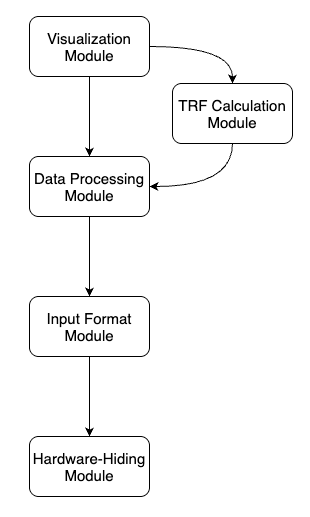
\includegraphics[width=0.4\textwidth]{UseHierarchy.png}
\caption{Use hierarchy among modules}
\label{FigUH}
\end{figure}

%\section*{References}

\section{User Interfaces}

Live Neuro provides a user interface with features such as:

\begin{itemize}
\item Data plotting of MEG/EEG data


\item Calculation of statistical index


\item Linking between multiple plots.


\end{itemize}


\section{Design of Communication Protocols}

Live Neuro modules communicate via structured API calls, allowing for efficient data flow between processing and visualization components.



\section{Timeline}

The development schedule follows an agile approach, with iterative testing and refinement. A GitHub repository will be used for version control and issue tracking.
The deadline for the Input Format Module, Data Processing Module, Visualization Module is March 18, March 22, and April 1, respectively.


\bibliographystyle {plainnat}
\bibliography{../../../refs/References}

\newpage{}

\end{document}